%%%%%%%%%%%%%%%%%%%%%%%%%%%%%%%%%%%%%%%%%%%%%%%
% Homotopy Type Theory
% Steve Awodey
% ICLA 2015
%%%%%%%%%%%%%%%%%%%%%%%%%%%%%%%%%%%%%%%%%%%%%

\documentclass[11pt]{article}
\usepackage{amsmath}
\usepackage{amssymb,latexsym}
\usepackage{amsthm}
\usepackage{bm}
%\input{prooftree}
\usepackage[all,cmtip]{xy}
\CompileMatrices       
\usepackage{url}
\xyoption{2cell}
\xyoption{curve}
\UseTwocells
\input{diagxy}  
\usepackage{tikz}
\usepackage{pdfpages}
\usepackage{bussproofs}
 

\newcommand{\toarrow}{\ensuremath{\rightarrow}} 
\newcommand{\T}{\ensuremath{\mathbb{T}}} 
\newcommand{\A}{A_\bullet}
\newcommand{\Id}{\mathrm{Id}}
\newcommand{\myemph}[1]{\textbf{#1}}    % Produces boldface text
\newcommand{\imp}{\ensuremath{\Rightarrow}} 
\newcommand{\arr}{\ensuremath{\rightarrow}} 


%%%
%%%  TYPE THEORETIC COMMANDS
%%%

\newcommand{\U}{\mathcal{U}}      
\newcommand{\Sn}{\mathbb{S}}       
\newcommand{\Z}{\mathbb{Z}}       
\newcommand{\rec}{\mathsf{rec}}    
\newcommand{\lloop}{\mathsf{loop}}    
\newcommand{\base}{\mathsf{base}}   
\newcommand{\cov}{\mathsf{cov}}   
\newcommand{\suc}{\mathsf{succ}}   
\newcommand{\ua}{\mathsf{ua}}    
\newcommand{\type}{\texttt{type}}       
\newcommand{\id}[1]{\texttt{Id}_{#1}} 
\newcommand{\judge}[3][]{#2\;\vdash_{#1}\;#3}

%%%%%%%%%%%%%%%%%%%%%%%%%%%%%%%%%%%%%%%%%%%%%%%%%%%%%%%%%%%%
\begin{document}
%%%%%%%%%%%%%%%%%%%%%%%%%%%%%%%%%%%%%%%%%%%%%%%%%%%%%%%%%%%%


%%
%% THEOREM LIKE ENVIRONMENT SETTINGS
%%

% theorem styles
\newtheorem{theorem}{Theorem}
\newtheorem*{theorem*}{Theorem}
\newtheorem{proposition}[theorem]{Proposition} 
\newtheorem{lemma}[theorem]{Lemma}
\newtheorem{corollary}[theorem]{Corollary} 

\theoremstyle{remark}
\newtheorem{remark}[theorem]{Remark} 
\newtheorem*{remarks*}{Remarks}
\newtheorem{example}[theorem]{Example}

\theoremstyle{definition}
\newtheorem{definition}[theorem]{Definition}


%%%%%%%%%%%%%%%%%%%%%%%%%%%%%%%%%%%%%%%%%%%%%%%%%%%%%%%%%%%%
%\begin{document}
%%%%%%%%%%%%%%%%%%%%%%%%%%%%%%%%%%%%%%%%%%%%%%%%%%%%%%%%%%%%

\title{
Homotopy Type Theory
}
\author{
Steve Awodey\thanks{
Partially supported by the U.S. Air Force Office of Sponsored Research.
}
}
\date{
Carnegie Mellon University\\
awodey@cmu.edu
}

\maketitle

\begin{abstract}
Homotopy Type Theory is a new, homotopical interpretation of constructive type theory.  It forms the basis of the recently proposed Univalent Foundations of Mathematics program. Combined with a computational proof assistant, and including a new foundational axiom -- the Univalence Axiom -- this program has the potential to shift the theoretical foundations of mathematics and computer science, and to affect the practice of working scientists. This talk will survey the field and report on some of the recent developments.
\end{abstract}

%%%%%%%%%%%%%%%%%%%%%%%%%%%%%%%%%%%%%%%%%%%%%%%%%%%%%%%%%
\subsection*{Overview}

\begin{itemize}
\item \emph{Homotopy Type Theory} is a recently discovered connection between Logic and Topology.  
%%\pause 
\item It is based on an interpretation of intensional Martin-L\"of type theory into homotopy theory.
%\pause 
\item \emph{Univalent Foundations} is an ambitious new program of foundations of mathematics based on HoTT.  
%\pause 
\item New constructions based on homotopical intuitions are added as Higher Inductive Types, providing classical spaces, (higher) quotients, truncations, etc.
%\pause 
\item The new Univalence Axiom is also added.  It implies that isomorphic structures are equal, in a certain sense.
%This makes the system more powerful logically and also more interesting philosophically.

\item And a new ``synthetic" style of axiomatics is used, simplifying and shortening  many proofs.
%\pause 
\item A large amount of classical mathematics has been developed in this new system:  basic homotopy theory, higher category theory, real analysis, commutative algebra, cumulative hierarchy of set theory, \dots .
%\pause
\item Proofs are formalized and verified in computerized proof assistants (e.g.\ Coq).
%\pause
\item There is a comprehensive book containing the informal development.
\end{itemize}

%%%%%%%%%%%%%%%%%%%%%%%%%%%%%%%%%%%%%%%%%%%%%%%%%%%%%%%%%
%\begin{frame}{Introduction}
%
%Homotopy type theory is an interpretation of intensional Martin-L\"of type theory into homotopy theory.
%%\pause 
%
%\begin{itemize}
%%\item \emph{Homotopy Type Theory}
%% \begin{itemize}
%\item Homotopy can be used to construct models of systems of constructive logic.
%%\pause
%\item Constructive type theory can be used as a formal calculus to reason about homotopy.
%%\pause
%\item The computational implementation of type theory allows computer verified proofs in homotopy theory, and elsewhere.
%%\pause
%\item The homotopical interpretation suggests some new logical constructions and axioms.
%\end{itemize}
%%\pause
%
%\emph{Univalent Foundations} combines these into a new program for foundations of mathematics.
%
%%The \emph{Univalence Axiom} is a new principle of reasoning.
%%\end{itemize}
%%\end{itemize}
%
%\end{frame}
%%%%%%%%%%%%%%%%%%%%%%%%%%%%%%%%%%%%%%%%%%%%%%%%%%%%%%%%%
\subsection*{Type theory}

Martin-L\"of constructive type theory consists of:
%
%\pause
\begin{itemize}
\item \myemph{Types}: $X, Y, \ldots, A\times B,\ A\rightarrow B, \ldots$
%\pause
\item \myemph{Terms}: $x: A,\ b: B,\ \langle a,b\rangle,\ \lambda x. b(x), \ldots$
%\pause
\item \myemph{Dependent Types}: $x:A\vdash B(x)$
%\begin{itemize}
%	%\pause \item $x:A, y:B(x)\vdash C(x,y)$
%	%\pause\item $x:A\vdash \sum_{y:B(x)} C(x,y)$
%	%\pause\item $x:A\vdash \prod_{y:B(x)} C(x,y)$
%	\end{itemize}
%\pause
\begin{itemize}
	\item $x:A, y:B(x)\vdash C(x,y)$
	\item $\sum_{x:A} B(x)$
	\item $\prod_{x:A} B(x)$
	\end{itemize}	
	%\pause
\item \myemph{Equations} $s = t : A$ %between terms of the same type, as in any algebraic theory.
\end{itemize}
%\pause
\medskip
%
%Formal calculus of typed terms and equations.
%%\pause
%
%Presented as a deductive system by rules of inference.
%%\pause

It was originally intended as a foundation for constructive mathematics, but is now used also in the theory of programming languages and as the basis of computational proof assistants.
%
%\end{frame}
%%%%%%%%%%%%%%%%%%%%%%%%%%%%%%%%%%%%%%%%%%%%%%%%%%%%%%%%%%%%%%%
%
%\begin{frame}{Type theory and homotopy}

%The dependent types are regarded as \myemph{indexed families of types}.  

%There are simple type forming operations $A\times B$ and $A\rightarrow B$, 

%And operations on dependent types including sum $\sum_{x:A}B(x)$ and product $\prod_{x:A}B(x)$ types.  There are also dependent terms and term-forming operations. 
%Finally, there are equations $s = t : A$ between terms of the same type, as in any algebraic theory.

%\end{frame}

%%%%%%%%%%%%%%%%%%%%%%%%%%%%
%\subsection{Curry-Howard}

\subsection*{Propositions as Types}

The system has a dual interpretation:
\begin{itemize}
\item once as \myemph{mathematical} objects: types are ``sets" and their terms are ``elements", which are being constructed,
%\pause
\item once as \myemph{logical} objects: types are ``propositions" and their terms are ``proofs", which are being derived.
\end{itemize}

%\pause
\medskip

This is known as the \myemph{Curry-Howard correspondence}:
\medskip

%\begin{align*}
%0,\ 1,\ A + B ,\ A\times B ,\ A\rightarrow B ,\ &\sum_{x:A} B(x) ,\ \prod_{x:A} B(x)\\
%\bot,\ \mathsf{T},\ A \vee B ,\ A\wedge B ,\ A\Rightarrow B ,\ &\exists_{x:A} B(x) ,\ \forall_{x:A} B(x)
%\end{align*}

\begin{tabular}{|c|c|c|c|c|c|c|}
\hline
$0$ & $1$ & $A + B$ & $A\times B$ & $A\rightarrow B$ & $\sum_{x:A} B(x)$ & $\prod_{x:A} B(x)$\\[1ex]
\hline 
$\bot$ & $\mathsf{T}$ & $A \vee B$ & $A\wedge B$ & $A\Rightarrow B$ & $\exists_{x:A} B(x)$ & $\forall_{x:A} B(x)$\\
\hline
\end{tabular}

\bigskip
%\pause

Gives the system its \myemph{constructive character}.

%\begin{tabular}{ccccccc}

%$0$ & $1$ & $A + B$ & $A\times B$ & $A\rightarrow B$ & $\sum_{x:A} B(x)$ & $\prod_{x:A} B(x)$\\
%\hline
%$\bot$ & $\mathsf{T}$ & $A \vee B$ & $A\wedge B$ & $A\Rightarrow B$ & $\exists_{x:A} B(x)$ & $\forall_{x:A} B(x)$\\

%\end{tabular}




\subsection*{Identity types}
%According to the logical interpretation we have:
%\begin{itemize}
%\item \myemph{propositional logic}: $A + B,\ A\times B,\ A\rightarrow B$,
%\item \myemph{predicate logic}: $B(x), C(x, y)$, with \myemph{quantifiers} $\prod$ and $\sum$.
%\end{itemize}
%
%%\pause

It's natural to add a primitive relation of \myemph{identity} between any terms of the same type:
\[
x, y:A \vdash \id{A}(x, y)
\]
\myemph{Logically} this is the proposition ``x is identical to y".
%\pause

But what is it \myemph{mathematically}?
%\pause

\medskip
%On the \myemph{mathematical} side, the identity type admits a newly discovered ``geometric" interpretation.
%
%\end{frame}
%%%%%%%%%%%%%%%%%%%%%%%%%%%%%
%
%\begin{frame}{Rules for identity types}
%
The \myemph{introduction} rule says that $a:A$ is always identical to itself:

\begin{prooftree}
  \AxiomC{$\mathtt{r}(a):\id{A}(a,a)$}
\end{prooftree}
\medskip

%\pause

The \myemph{elimination} rule is a form of Lawvere's law:

\begin{prooftree}
 \AxiomC{$c:\id{A}(a,b)$}
  \AxiomC{$\judge{x:A}{d(x):R\bigl(x,x,\mathtt{r}(x)\bigr)}$}
  \BinaryInfC{$\mathtt{J}_d(a,b,c):R(a,b,c)$}
\end{prooftree}
\medskip
%\pause
Schematically:
\[
``\ a=b\  \&\ R(x,x)\  \Rightarrow\ R(a,b)\ "
\]
%%\pause
%The identity type admits a \myemph{geometric interpretation}.

%There is a book-keeping condition on proof terms:

%\begin{prooftree}
%  %\AxiomC{$a:A$}
% % \RichtLabel{conversion}
%  \AxiomC{$\mathtt{J}_d\bigl(a,a,\mathtt{r}a\bigr)\;=\;d(a)$}
%\end{prooftree}
%\medskip

%\end{frame}

%%%%%%%%%%%%%%%%%%%%%%%%%%%%%%%%%%%%%%%%%%%%%%%%%%%%%%%%%%%%%%%%
%
%\begin{frame}{Intensionality}
%
%The rules are such that if $a$\/ and $b$\/ are \myemph{equal} as terms: 
%\[
%a=b\]
%then they are also logically \myemph{identical}: 
%\[
%t : \id{A}(a,b)\quad \text{(for some $t$)}.
%\]
%
%\begin{itemize}%\pause
%\item But the converse is not true --- this is called \myemph{intensionality}.
%%\pause
%\item Terms that are identified logically may nonetheless remain distinct syntactically --- e.g.\  different expressions may determine ``the same" function.
%%\pause
%\item Allowing such distinctions gives the system good computational and proof-theoretic properties.
%%\pause
%\item It also gives rise to a structure of great combinatorial complexity.
%\end{itemize}
%\end{frame}
%%
%%%%%%%%%%%%%%%%%%%%%%%%
%\subsection{The homotopy interpretation (I)}
%%%%%%%%%%%%%%%%%%%%%%%%

\subsection*{The homotopy interpretation (Awodey-Warren)}

Suppose we have terms of ascending identity types:
\begin{align*}
  a,\ b :&\ A     \\ 
  p,\ q :&\ \id{A}(a, b)    \\ 
   \alpha,\ \beta :&\ \id{\id{A}(a,b)}{(p, q)}   \\ 
 \ldots :&\ \id{\id{\id{\ldots}}}{(\ldots)}   
\end{align*}

%\pause
Consider the following interpretation:
%
\begin{align*}
\text{Types} &\quad\leadsto\quad  \text{Spaces} \\
\text{Terms} &\quad\leadsto\quad  \text{Maps} \\
a : A &\quad\leadsto\quad  \text{Points $a : 1 \rightarrow A$} \\
p : \id{A}(a, b) &\quad\leadsto\quad  \text{Paths $p: a \Rightarrow b$} \\
\alpha : \id{\id{A}(a, b)}(p, q) &\quad\leadsto\quad  \text{Homotopies $\alpha: p\Rrightarrow q$} \\
\vdots &
\end{align*}

%\end{frame}
%
%%%%%%%%%%%%%%%%%%%%%%%%%%%%%%%%%%%%%%%%%%%%%%%%%%%%%%%%%%%%%%%%
%
%\begin{frame}{The homotopy interpretation (Awodey-Warren)}

This extends the familiar \myemph{topological interpretation} of the \emph{simply-typed} $\lambda$-calculus: 
\begin{align*}
\text{types} &\leadsto \text{spaces}\\
\text{terms} &\leadsto \text{continuous functions}
 \end{align*}

%\pause

to \emph{dependently typed} $\lambda$-calculus with $\id{}$-types, via the \myemph{basic idea}:
\[
p : \id{X}(a,b)\ \leadsto\ \text{$p$ is a path from point $a$ to point $b$ in $X$}
\]

%\pause
This forces \emph{dependent types to be fibrations}, 
$\id{}$\emph{-types to be path spaces}, and \emph{homotopic maps to be identical}.

\subsection*{The fundamental groupoid of a type (Hofmann-Streicher)}

Like path spaces in topology, identity types endow each type in the system with the structure of a (higher-) groupoid:
$$
\begin{array}{c}
\begin{array}{cccc}
\ \xy
(0,0)*{\bullet};
(0,80)*{a};
\endxy \quad
&
\ \xy
(0,0)*{\bullet}="a";
(0,80)*{\scriptstyle a};
(400,0)*{\bullet}="b";
(400,80)*{\scriptstyle b};
{\ar "a";"b"};
(200,80)*{p};
\endxy \ 
&
\ \xy
(0,0)*+{\bullet}="a";
(0,80)*{\scriptstyle a};
(450,0)*+{\bullet}="b";
(450,80)*{\scriptstyle b};
{\ar@/^1pc/^{p} "a";"b"};
{\ar@/_1pc/_{q} "a";"b"};
{\ar@{=>} (210,85)*{};(210,-85)*{}};
(280,0)*{\alpha};
\endxy \ 
&
\xy 0;/r.22pc/: 
(0,15)*{}; 
(0,-15)*{}; 
(0,8)*{}="A"; 
(0,-8)*{}="B"; 
%{\ar@{=>} "A" ; "B"}; 
{\ar@{=>}@/_.75pc/ "A"+(-4,1) ; "B"+(-3,0)}; 
(-10,0)*{\alpha};
{\ar@{=}@/_.75pc/ "A"+(-4,1) ; "B"+(-4,1)}; 
{\ar@{=>}@/^.75pc/ "A"+(4,1) ; "B"+(3,0)}; 
(10,0)*{\beta};
{\ar@{=}@/^.75pc/ "A"+(4,1) ; "B"+(4,1)}; 
{\ar@3{->} (-6,0)*{} ; (6,0)*+{}}; 
(0,4)*{\vartheta};
%{\ar@3{->} (2,0)*{} ; (6,0)*+{}}; 
(-15,0)*+{\bullet}="1"; 
(-15,4)*{\scriptstyle a};
(15,0)*+{\bullet}="2"; 
(15,4)*{\scriptstyle b};
{\ar@/^2.75pc/^{p} "1";"2"}; 
{\ar@/_2.75pc/_{q} "1";"2"}; 
\endxy
\end{array} 
\end{array}
$$
%\end{frame}
%
%%%%%%%%%%%%%%%%%%%%%%%%%%%%%%%%%%%%%%%%%%%%%%%%%%%%%%%%%%%%%%%%
%
%\begin{frame}{Fundamental groupoids}
%
%As in topology, the terms of order 0 and 1, (``points" and ``paths"),
%$$
%\begin{array}{c}
%\ \xy
%(0,0)*{\bullet}="a";
%(0,80)*{\scriptstyle a};
%(400,0)*{\bullet}="b";
%(400,80)*{\scriptstyle b};
%{\ar "a";"b"};
%(200,80)*{p};
%\endxy \ 
%\end{array}
%$$
%
%bear the structure of a \myemph{groupoid}.  
%
%\pause
%\smallskip
The laws of identity are the \myemph{groupoid operations}:
%
\begin{align*}
r : \id{}(a,a) &\qquad \text{reflexivity} && a \rightarrow a \\
s: \id{}(a,b)\rightarrow\id{}(b,a) &\qquad \text{symmetry} && a \leftrightarrows b \\
t :  \id{}(a,b)\times\id{}(b,c)\rightarrow\id{}(a,c) &\qquad \text{transitivity} && a \rightarrow b \rightarrow c
\end{align*}
%
%\pause
The \myemph{groupoid equations} only hold ``up to homotopy", i.e.\ up to a higher identity term.
%\end{frame}

%%%%%%%%%%%%%%%%%%%%%%%%%%%%%%%%%%%%%%%%%%%%%%%%%%%%%%%%%%%%%%%%
%
%\begin{frame}{The fundamental groupoid of a type}
%
%But also just as in topology, the \myemph{groupoid equations} of associativity, inverse, and unit:
%\begin{align*}
%p\cdot(q\cdot r) &= (p\cdot q)\cdot r\\
% p^{-1}\cdot p = &\ 1 = p\cdot p^{-1}\\
%1\cdot p = &\ p = p\cdot 1
%\end{align*}
%do not hold strictly, but only ``up to homotopy".
%
%%\pause
%\medskip
%This means they are witnessed by terms of the next higher order:
%\[
%\vartheta :  \id{\id{}}\left(p^{-1}\cdot p, 1\, \right)
%\]
%$$
%\begin{array}{c}
%\ \xy
%(0,0)*+{\bullet}="a";
%(-80,0)*{\scriptstyle a};
%(450,400)*+{\bullet}="b";
%(450,480)*{\scriptstyle b};
%(900,0)*+{\bullet}="c";
%(980,0)*{\scriptstyle a};
%{\ar@/^1pc/^{p} "a";"b"};
%{\ar@/^1pc/^{p^{-1}} "b";"c"};
%{\ar@/_1pc/_{1} "a";"c"};
%{\ar@{=>} (450,300)*{};(450,0)*{}};(350,200)*{\vartheta};
%\endxy \ 
%\end{array}
%$$
%
%\end{frame}
%%%%%%%%%%%%%%%%%%%%%%%%%%%%%%%%%%%%%%%%%%%%%%%%%%%%%%%%%%%%%%%
%\begin{frame}{Fundamental groupoids}
%
%The entire system of identity terms of all orders forms an infinite-dimensional graph, or ``globular type":
%\[
%A \leftleftarrows \id{A}  \leftleftarrows \id{\id{A}} \leftleftarrows \id{\id{\id{A}}} \leftleftarrows \ldots
%\]
%
%%\pause
%
%It has the structure of an internal (weak), infinite-dimensional, groupoid, as occurring homotopy theory:
%
%\medskip
%
%\begin{theorem}[Lumsdaine, Garner \& van den Berg, 2009]
%The system of identity terms of all orders over any fixed type is a weak $\infty$-groupoid.
%\end{theorem}
%
%%\pause
%
%\medskip
%
%Every type has a \myemph{fundamental weak $\infty$-groupoid}.
%
%\end{frame}
%%%%%%%%%%%%%%%%%%%%%%%%%%%%%%%%%%%%%%%%%%%%%%%%%%%%%%%%%%%%%%%
%
%\begin{frame}{The homotopy interpretation (I)}
%
%This \myemph{homotopy interpretation} captures a certain \myemph{logic of homotopy} that was not previously formalized.
%
%%\pause
%\medskip
%
%The system of type theory can be used to reason \myemph{formally} about homotopy.
%%\pause
%\medskip
%
%We still need to interpret \myemph{dependent types} and \myemph{identity types}.
%
%\end{frame}
%
%%%%%%%%%%%%%%%%%%%%%%%%%%%%%%%%%%%%%%%%%%%%%%%%%%%%%%%%
%\subsubsection{Rules for identity types}
%\strut
%\bigskip
%
%\begin{frame}{Rules for identity types}
%
%\begin{prooftree}
%  \AxiomC{$A:\type$}
%  \RightLabel{$\id{}$ formation}
%  \UnaryInfC{$\judge{x,y:A}{\id{A}{}(x,y):\type}$}
%\end{prooftree}
%\smallskip
%
%%\pause
%
%\begin{prooftree}
%  \AxiomC{$a:A$}
%  \RightLabel{$\id{}$ introduction}
%  \UnaryInfC{$\mathtt{r}(a):\id{A}(a,a)$}
%\end{prooftree}
%\medskip
%
%%\pause
%
%\begin{prooftree}
%  \AxiomC{$\judge{x, y:A,z:\id{A}(x,y)}{B(x,y,z):\type}$}
%  \noLine
%  \UnaryInfC{$\judge{x:A}{b(x):B\bigl(x,x,\mathtt{r}(x)\bigr)}$}
%  \RightLabel{$\id{}$ elimination}
%  \UnaryInfC{$\judge{x, y:A,z:\id{A}(x,y)}{\mathtt{J}(b,x,y,z):B(x,y,z)}$}
%\end{prooftree}
%\smallskip
%
%%\pause
%
%\begin{prooftree}
%  \AxiomC{$a:A$}
%  \RightLabel{$\id{}$ conversion}
%  \UnaryInfC{$\mathtt{J}\bigl(b,a,a,\mathtt{r}(a)\bigr)\;=\;b(a):B\bigl(a,a,\mathtt{r}(a)\bigr)$}
%\end{prooftree}
%\medskip
%
%%The introduction rule provides a witness $\mathtt{r}(a)$ that $a$ is identical to itself, called the \emph{reflexivity term}. 
%%The distinctive elimination rule can be recognized as a form of Leibniz's law.
%
%\end{frame}
%

%%%%%%%%%%%%%%%%%%%%%%%%%%%%%%%%%%%%%%%%%%%%%%%%%%%%%%%%%%%%%%%%
%
%\begin{frame}{The homotopy interpretation: Type dependency}
%
%We still need to interpret dependent types $x:A\ \vdash B(x)$.
%%\pause
%
%The identity rules imply the following:
%%\pause
%
%\begin{prooftree}
% % \AxiomC{$x : A \vdash B(x)$}
%  \AxiomC{$p : \id{A}(a,a^\prime)$}
%  \AxiomC{$b : B(a)$}
%%   \UnaryInfC{$x : A, y : B(x) \vdash y : B(x)$}
%%   \UnaryInfC{$x : A \vdash \lambda y.y : B(x) \rightarrow B(x)$}
%%  \BinaryInfC{$p_*: B(a) \rightarrow B(b)$}
%  \BinaryInfC{$p_*b: B(a^\prime)$}
%\end{prooftree}
%
%%\pause
%Logically, this just says ``$a = a^\prime\ \&\ B(a) \Rightarrow B(a^\prime)$".
%%\pause
%\medskip
%
%But topologically, it is a familiar \myemph{lifting property}:
%\[
%\xymatrix{
%B  \ar[d] & b  \ar@{..>}[r] &  p_*b \\
%A & a  \ar[r]_{p} & a^\prime
%}
%\]
%
%%\pause
%This is the notion of a ``fibration'' of spaces.
%\end{frame}
%
%%%%%%%%%%%%%%%%%%%%%%%%%%%%%%%%%%%%%%%%%%%%%%%%%%%%%%%%%%%%%%%%
%
%\begin{frame}{The homotopy interpretation: Type dependency}
%
%Thus we continue the homotopy interpretation as follows:
%%
%\[
%\text{Dependent types\quad $x:A \vdash B(x)$} \quad\leadsto\quad  \text{Fibrations}\quad \xymatrix{ B \ar[d]\\
% A}\]
% 
%%\pause
%
%The type $B(a)$ is the fiber of $B\toarrow A$ over the point $a : A$
%%
%\[
%\xymatrix{
%B(a) \ar[d] \ar[r] & B  \ar[d]\\
%1 \ar[r]_{a\ } & A.
%}
%\]
% 
%%
%\end{frame}
%%%%%%%%%%%%%%%%%%%%%%%%%%%%%%%%%%%%%%%%%%%%%%%%%%%%%%%%%%%%%%%%
%
%\begin{frame}{The homotopy interpretation: Identity types}
%
%To interpret the identity type $x, y:A \vdash \id{A}(x,y)$, we thus require a fibration over $A\times A$.  
%%\pause
%
%Take the space $A^I$ of all paths in $A$:
%\[
%\text{Identity type\quad $x, y:A \vdash \id{A}(x,y)$} \quad\leadsto\quad  \text{Path space}\quad \xymatrix{ A^I\ar[d]\\
% A\times A}\]
%
%%\pause
%
%The fiber $\id{A}(a,b)$ over a point $(a,b)\in A\times A$ is the space of paths from $a$ to $b$ in $A$.
%%
%\[
%\xymatrix{
%\id{A}(a,b) \ar[d] \ar[r] & A^I  \ar[d]\\
%1 \ar[r]_{(a,b)\ } & A\times A.
%}
%\]
%
%\end{frame}
%
%%%%%%%%%%%%%%%%%%%%%%%%%%%%%%%%%%%%%%%%%%%%%%%%%%%%%%%%%%%%%%%%%%%%%%%%%%%%%%%%%%%%%%%%%
%
%\begin{frame}{The homotopy interpretation: Identity types}
%
%The path space $A^I$ classifies homotopies $\vartheta : f\Rightarrow g$ between maps $f, g : X\rightarrow A$,
%\[
%\xymatrix{
%&& A^I  \ar[d] \\
%X \ar[rru]^{\vartheta} \ar[rr]_{(f, g)} && A\times A.
%}
%\]
%
%%\pause
%\medskip
%
%So given any terms $x : X \vdash f, g : A$, an identity term $$x: X \vdash \vartheta : \id{A}(f,g)$$ is interpreted as a \myemph{homotopy} between $f$ and $g$.
%
%\end{frame}
%
%%%%%%%%%%%%%%%%%%%%%%%%%%
%%\subsection{The homotopy interpretation (II)}
%%%%%%%%%%%%%%%%%%%%%%%%%%
%%%%%%%%%%%%%%%%%%%%%%%%%%%%%%%%%%%%%%%%%%%%%%%%%%%%%%%%%%%%%%%%
%
%\begin{frame}{The homotopy interpretation: Summary}
%
%\begin{enumerate}
%\item There is a \myemph{topological interpretation} of the  $\lambda$-calculus: 
%\begin{align*}
%\text{types} &\leadsto \text{spaces}\\
%\text{terms} &\leadsto \text{continuous functions}\\
% &\ldots \\
%\text{computability} &\leadsto  \text{continuity}
%\end{align*}
%
%%\pause
%\medskip
%
%\item Extend this to dependently typed $\lambda$-calculus with $\id{}$-types, \\
%%\pause using the \myemph{basic idea}:
%\[\begin{split}
%p : \id{X}(a,b)\ &\Leftrightarrow  \\
% &\text{$p$ is a path from point $a$ to point $b$ in the space $X$}
%\end{split}\]
%%\pause
%This forces dependent types to be fibrations, %\pause $\id{}$-types to be path spaces, %\pause and terms of $\id{}$-types to be homotopies.
%
%\end{enumerate}
%
%\end{frame}
%%%%%%%%%%%%%%%%%%%%%%%%%%%%%%%%%%%%%%%%%%%%%%%%%%%%%%%%%%%%%%%%%%%%%%%%%%%%%%%%%%%%%%%%%%%%%%%%%%%%%%%%%%%%%%%%%%%%%%%%%%%%%%%
%
%\begin{frame}{The homotopy interpretation: First theorems}
%
%Instead of concrete spaces and homotopies, we use the axiomatic description provided by \myemph{Quillen model categories}.  
%
%%\pause
%\begin{itemize}
%\item Gives a wide range of different models.
%%\pause
%\item Includes classical homotopy of spaces and simplicial sets.
%%\pause
%\item Allows the use of standard methods from categorical logic.
%\end{itemize}
%
%%\pause
%\begin{theorem}[Awodey \& Warren 2006]
%``Martin-L\"of type theory has a \myemph{sound} interpretation into abstract homotopy theory."
%\end{theorem}
%
%%\pause
%\medskip
%
%\begin{theorem}[Gambino \& Garner 2008]
%``The homotopy interpretation of Martin-L\"of type theory is also \myemph{complete}."
%\end{theorem}
%
%%%\pause
%%\medskip
%
%%More precisely:  in the theory of identity, a judgement that is valid under every coherent interpretation in a weak factorization system is also provable.
%
%%%\pause
%%\medskip
%
%%The proof uses the standard method of \emph{syntactic categories} to construct a canonical model.
%
%\end{frame}
%
%%%%%%%%%%%%%%%%%%%%%%%%%%%%%%%%%%%%%%%%%%%%%%%%%%%%%%%%%%%%%%%%%
%
%%\begin{frame}{Theorem 2}
%
%%\begin{theorem}[Garner \& Gambino 2009]
%%The homotopy interpretation of Martin-L\"of type theory is essentially \myemph{complete} with respect to models in weak factorization systems. 
%%\end{theorem} 
%
%%%\bigskip
%%%%\pause
%
%%%\noindent There is a technical issue of selecting path objects $A^I$ and diagonal fillers $j$ as interpretations of $\id{A}$-types and $\mathtt{J}$-terms in a ``coherent" way, i.e.\ respecting substitution of terms for variables; various solutions are available.  Being able to prove this fundamental result is the second reason for using \emph{abstract} homotopy for our semantics.
%
%%\end{frame}
%
%%%%%%%%%%%%%%%%%%%%%%%%%%%%%%%%%%%%%%%%%%%%%%%%%%%%%%%%%%%%%%%%%
%
%\begin{frame}{1. The homotopy interpretation: Conclusion}
%\medskip
%
%%Summing up this first half of the lecture, we have now seen that:
%
%\bigskip
%
%\begin{verse}
%\emph{Type theory provides a ``logic of homotopy".}
%\end{verse}
%
%\bigskip
%
%\end{frame}
%
%%%%%%%%%%%%%%%%%%%%%%%%%%%%%%%%%%%%%%%%%%%%%%%%%%%%%%%%%%%%%%%%
%%%%%%%%%%%%%%%%%%%%%%%%%%%%%%%%%%%%%%%%%%%%%%%%%%%%%%%%%
%\section{2. Homotopy type theory}
%%%
%%%%%%%%%%%%%%%%%%%%%%%%%%%%%%%%%%%%%%%%%%%%%%%%%%%
%
%\begin{frame}{2. Homotopy type theory}
%
%How \myemph{expressive} is constructive type theory as a formal language for homotopy theory?  
%
%\medskip
%%\pause
%
%What facts, properties, and constructions from homotopy theory are logically expressible?
%
%\medskip
%%\pause
%
%One example: the \myemph{fundamental group} and its higher-dimensional analogues are logical constructions.
%%
%\end{frame}
%%%%%%%%%%%%%%%%%%%%%%%%%%%%%%%%%%%%%%%%%%%%%%%%%%%%%%%%%%%%%%%%
%%%%%%%%%%%%%%%%%%%%%%%%%%%%%%%%%%%%%%%%%%%%%%%%%%%%%%%%%%%%%%%%
%
%\begin{frame}{The fundamental groupoid of a type}
%
%But also just as in topology, the \myemph{groupoid equations} of associativity, inverse, and unit:
%\begin{align*}
%p\cdot(q\cdot r) &= (p\cdot q)\cdot r\\
% p^{-1}\cdot p = &\ 1 = p\cdot p^{-1}\\
%1\cdot p = &\ p = p\cdot 1
%\end{align*}
%do not hold strictly, but only ``up to homotopy".
%
%%\pause
%\medskip
%This means they are witnessed by terms of the next higher order:
%\[
%\vartheta :  \id{\id{}}\left(p^{-1}\cdot p, 1\, \right)
%\]
%$$
%\begin{array}{c}
%\ \xy
%(0,0)*+{\bullet}="a";
%(-80,0)*{\scriptstyle a};
%(450,400)*+{\bullet}="b";
%(450,480)*{\scriptstyle b};
%(900,0)*+{\bullet}="c";
%(980,0)*{\scriptstyle a};
%{\ar@/^1pc/^{p} "a";"b"};
%{\ar@/^1pc/^{p^{-1}} "b";"c"};
%{\ar@/_1pc/_{1} "a";"c"};
%{\ar@{=>} (450,300)*{};(450,0)*{}};(350,200)*{\vartheta};
%\endxy \ 
%\end{array}
%$$
%
%\end{frame}
%%%%%%%%%%%%%%%%%%%%%%%%%%%%%%%%%%%%%%%%%%%%%%%%%%%%%%%%%%%%%%%%
%\begin{frame}{Fundamental groupoids}
%
%The entire system of identity terms of all orders forms an infinite-dimensional graph, or ``globular set":
%\[
%A \leftleftarrows \id{A}  \leftleftarrows \id{\id{A}} \leftleftarrows \id{\id{\id{A}}} \leftleftarrows \ldots
%\]
%
%%\pause
%
%It has the structure of a (weak), infinite-dimensional, groupoid, as already occurring homotopy theory:
%
%\medskip
%
%\begin{theorem}[Lumsdaine, Garner \& van den Berg, 2009]
%The system of identity terms of all orders over any fixed type is a weak $\infty$-groupoid.
%\end{theorem}
%
%%\pause
%
%\medskip
%
%Every type has a \myemph{fundamental weak $\infty$-groupoid}.
%
%\end{frame}
%%%%%%%%%%%%%%%%%%%%%%%%%%%%%%%%%%%%%%%%%%%%%%%%%%%%%%%%%%%%%%%%
\subsection*{Homotopy $n$-types (Voevodsky)}

The universe of all types is  stratified by ``homotopical dimension": the level at which the fundamental groupoid becomes trivial.
%\pause
\medskip

A type $X$ is called:
\begin{description}
\item[contractible] iff \quad $\sum_{x:X}\prod_{y:X}\id{X}(x,y)$
\end{description}
\medskip
%\pause

A type $X$ is a:
\begin{description}
\item[proposition] iff \quad $\prod_{x,y:X}\ \mathsf{Contr}(\id{X}(x,y))$,%\pause
\item[set] iff \quad $\prod_{x,y:X}\ \mathsf{Prop}(\id{X}(x,y))$,%\pause
\item[$1$-type] iff \quad $\prod_{x,y:X}\ \mathsf{Set}(\id{X}(x,y))$,%\pause
\item[(n+1)-type] iff \quad $\prod_{x,y:X}\ \mathsf{nType}(\id{X}(x,y))$.
\end{description}
%\pause
\medskip

This gives a new view of the mathematical universe.
%\end{frame}
%%%%%%%%%%%%%%%%%%%%%%%%%%%%%%%%%%%%%%%%%%%%%%%%%%%%%%%%%%%%%%%%%
%\begin{frame}{Machine implementation}
%
%%Answer to the question \emph{``How much homotopy theory can be expressed in this type theory?"} is:
%%%\pause
%%\myemph{a lot!}
%%%\pause
%%
%%\medskip
%Now one can combine the following:
%
%%\pause
%\begin{itemize}
%
%\item the representation of homotopy theory in constructive type theory
%%\pause
%
%\item the well-developed implementations of type theory in computational proof assistants like Coq.
%\end{itemize}
%%\pause
%
%Allows computer verified proofs in homotopy theory and related fields, in addition to constructive mathematics.
%%\pause
%\medskip
%
%This aspect is being very actively pursued right now in the Univalent Foundations Program.
%%\medskip
%%This is the starting point of the \emph{Univalent Foundations Program}.
%
%\end{frame}
%
%%%%%%%%%%%%%%%%%%%%%%%%%%%%%%%%%%%%%%%%%%%%%%%%%%%%%%%%%%%%%%%%%%
%%%
%\begin{frame}{A computational example}
%
%A classical result states that the higher homotopy groups of a space are always abelian.
%%\pause
%
%We can formalize this in type theory:
%%\pause
%\begin{itemize}
%\item the fundamental group  $\pi_1(X,b)$ of a type $X$ at basepoint $b : X$ consists of terms of type $\id{X}(b, b)$.
%%\pause
%\item the second homotopy group  $\pi_2(X,b)$ consists of terms of type $\id{\id{X}(b, b)}(\mathtt{r}(b), \mathtt{r}(b))$.
%%\pause
%\item Each of these types has a group structure, and so the second one has \emph{two} group structures that are compatible.
%%\pause
%\item Now the Eckmann-Hilton argument shows that the two structures on $\pi_2(X,b)$ agree, and are abelian.
%\end{itemize}
%%\pause
%
%This argument can be formalized in  Coq and verified to be correct.
%In this way, we can use the homotopical interpretation to verify proofs in homotopy theory.
%
%\end{frame}
%
%%%%%%%%%%%%%%%%%%%%%%%%%%%%%%%%%%%%%%%%%%%%%%%%%%%%%%%%%%%%%%%%%
%%
%\begin{frame}[fragile]{A computational example}
%
%{\relsize{-15}
%\begin{verbatim}
%(** ** The 2-dimensional groupoid structure *)
%
%(** Horizontal composition of 2-dimensional paths. *)
%Definition concat2 {A} {x y z : A} {p p' : x = y} {q q' : y = z} (h : p = p') (h' : q = q') 
%: p @ q = p' @ q'
%:= match h, h' with idpath, idpath => 1 end.
%
%Notation ``p @@ q" := (concat2 p q)
%
%(** 2-dimensional path inversion *)
%Definition inverse2 {A : Type} {x y : A} {p q : x = y} (h : p = q) : p^ = q^
%:= match h with idpath => 1 end.
%
%(** *** Whiskering *)
%
%Definition whiskerL {A : Type} {x y z : A} (p : x = y) {q r : y = z} (h : q = r) : p @ q = p @ r
%:= 1 @@ h.
%
%Definition whiskerR {A : Type} {x y z : A} {p q : x = y} (h : p = q) (r : y = z) : p @ r = q @ r
%:= h @@ 1.
%
%(** *** Unwhiskering, a.k.a. cancelling. *)
%
%Lemma cancelL {A} {x y z : A} (p : x = y) (q r : y = z) : (p @ q = p @ r) -> (q = r).
%Proof.
%  destruct p, r. intro a. exact ((concat_1p q)^ @ a).
%Defined.
%
%Lemma cancelR {A} {x y z : A} (p q : x = y) (r : y = z) : (p @ r = q @ r) -> (p = q).
%Proof.
%  destruct r, p. intro a. exact (a @ concat_p1 q).
%Defined.
%\end{verbatim}
%}
%
%\end{frame}
%%%%%%%%%%%%%%%%%%%%%%%%%%%%%%%%%%%%%%%%%%%%%%%%%%%%%%%%%
%\begin{frame}[fragile]
%
%{\relsize{-15}
%\begin{verbatim}
%(** Whiskering and identity paths. *)
%
%Definition whiskerR_p1 {A : Type} {x y : A} {p q : x = y} (h : p = q) :
%  (concat_p1 p) ^ @ whiskerR h 1 @ concat_p1 q = h
%  :=
%  match h with idpath =>
%    match p with idpath =>
%      1
%    end end.
%
%Definition whiskerR_1p {A : Type} {x y z : A} (p : x = y) (q : y = z) :
%  whiskerR 1 q = 1 :> (p @ q = p @ q)
%  :=
%  match q with idpath => 1 end.
%
%Definition whiskerL_p1 {A : Type} {x y z : A} (p : x = y) (q : y = z) :
%  whiskerL p 1 = 1 :> (p @ q = p @ q)
%  :=
%  match q with idpath => 1 end.
%
%Definition whiskerL_1p {A : Type} {x y : A} {p q : x = y} (h : p = q) :
%  (concat_1p p) ^ @ whiskerL 1 h @ concat_1p q = h
%  :=
%  match h with idpath =>
%    match p with idpath =>
%      1
%    end end.
%
%Definition concat2_p1 {A : Type} {x y : A} {p q : x = y} (h : p = q) :
%  h @@ 1 = whiskerR h 1 :> (p @ 1 = q @ 1)
%  :=
%  match h with idpath => 1 end.
%
%Definition concat2_1p {A : Type} {x y : A} {p q : x = y} (h : p = q) :
%  1 @@ h = whiskerL 1 h :> (1 @ p = 1 @ q)
%  :=
%  match h with idpath => 1 end.
%  \end{verbatim}
%}
%
%\end{frame}
%%%%%%%%%%%%%%%%%%%%%%%%%%%%%%%%%%%%%%%%%%%%%%%%%%%%%%%%%
%\begin{frame}[fragile]
%
%{\relsize{-15}
%\begin{verbatim}
%
%(** The interchange law for concatenation. *)
%Definition concat_concat2 {A : Type} {x y z : A} {p p' p'' : x = y} {q q' q'' : y = z}
%  (a : p = p') (b : p' = p'') (c : q = q') (d : q' = q'') :
%  (a @@ c) @ (b @@ d) = (a @ b) @@ (c @ d).
%Proof.
%  case d.
%  case c.
%  case b.
%  case a.
%  reflexivity.
%Defined.
%
%(** The interchange law for whiskering.  Special case of [concat_concat2]. *)
%Definition concat_whisker {A} {x y z : A} (p p' : x = y) (q q' : y = z) (a : p = p') (b : q = q') :
%  (whiskerR a q) @ (whiskerL p' b) = (whiskerL p b) @ (whiskerR a q')
%  :=
%  match b with
%    idpath =>
%    match a with idpath =>
%      (concat_1p _)^
%    end
%  end.
%
%(** Structure corresponding to the coherence equations of a bicategory. *)
%
%(** The "pentagonator": the 3-cell witnessing the associativity pentagon. *)
%Definition pentagon {A : Type} {v w x y z : A} (p : v = w) (q : w = x) (r : x = y) (s : y = z)
%  : whiskerL p (concat_p_pp q r s)
%      @ concat_p_pp p (q@r) s
%      @ whiskerR (concat_p_pp p q r) s
%  = concat_p_pp p q (r@s) @ concat_p_pp (p@q) r s.
%Proof.
%  case p, q, r, s.  reflexivity.
%Defined.
% \end{verbatim}
%}
%
%\end{frame}
%%%%%%%%%%%%%%%%%%%%%%%%%%%%%%%%%%%%%%%%%%%%%%%%%%%%%%%%%
%\begin{frame}[fragile]
%
%{\relsize{-15}
%\begin{verbatim}
%
%(** The 3-cell witnessing the left unit triangle. *)
%Definition triangulator {A : Type} {x y z : A} (p : x = y) (q : y = z)
%  : concat_p_pp p 1 q @ whiskerR (concat_p1 p) q
%  = whiskerL p (concat_1p q).
%Proof.
%  case p, q.  reflexivity.
%Defined.
%
%(** The Eckmann-Hilton argument *)
%Definition eckmann_hilton {A : Type} {x:A} (p q : 1 = 1 :> (x = x)) : p @ q = q @ p :=
%  (whiskerR_p1 p @@ whiskerL_1p q)^
%  @ (concat_p1 _ @@ concat_p1 _)
%  @ (concat_1p _ @@ concat_1p _)
%  @ (concat_whisker _ _ _ _ p q)
%  @ (concat_1p _ @@ concat_1p _)^
%  @ (concat_p1 _ @@ concat_p1 _)^
%  @ (whiskerL_1p q @@ whiskerR_p1 p).
%
%\end{verbatim}
%}
%
%\end{frame}
%
%%%%%%%%%%%%%%%%%%%%%%%%%%%%%%%%%%%%%%%%%%%%%%%%%%%%%%%%%%%%%%%%
%
%\begin{frame}{Homotopy type theory: Summary}
%
%\begin{itemize}
%
%\item Constructive type theory provides a logic of homotopy.
%%\pause
%
%\item Logical methods capture a lot of homotopy theory: e.g.\ the fundamental $\infty$-groupoid of a space is a \emph{logical construction}, and the notion of an $n$-type is \emph{logically definable}.
%%\pause
%
%\item Many results have already been formalized: homotopy groups of spheres, Freudenthal suspension theorem, Postnokov towers, Eilenberg--Mac Lane spaces,  ...
%%\pause
%
%\item Other areas are also being developed:
%
%\begin{itemize}
%	\item Foundations: quotient types, inductive types, cumulative hierarchy of sets, ...
%	%\pause
%	\item Elementary mathematics: basic algebra, real numbers, cardinal arithmetic, ...
%	\end{itemize}
%%\pause
%
%\item Some new logical ideas are suggested by the homotopy interpretation: Higher inductive types, Univalence axiom.
%
%\end{itemize}
%
%\end{frame}
%
%%%%%%%%%%%%%%%%%%%%%%%%%%%%%%%%%%%%%%%%%%%%%%%%%%%%%%%%%%%%%%%%
%\section{3. A new logical construction: Higher Inductive Types}
%%%%%%%
\subsection*{Higher inductive types (Lumsdaine-Shulman)}

The natural numbers $\mathbb{N}$ are implemented as an (ordinary) inductive type:
\[
			\mathbb{N} := \begin{cases} &0 : \mathbb{N}\\
		 				&s : \mathbb{N} \rightarrow \mathbb{N}
						\end{cases}
\]
%\pause
%
The \myemph{recursion property} is captured by an elimination rule:

\begin{prooftree}
% \AxiomC{$X$ type}
 \AxiomC{$a : X$}
  \AxiomC{$f : X \rightarrow X$}
%   \UnaryInfC{$x : A, y : B(x) \vdash y : B(x)$}
%   \UnaryInfC{$x : A \vdash \lambda y.y : B(x) \rightarrow B(x)$}
%  \BinaryInfC{$p_*: B(a) \rightarrow B(b)$}
  \BinaryInfC{$\mathsf{rec}(a,f) :  \mathbb{N} \rightarrow X$}
\end{prooftree}
%
%\pause

with computation rules:
\begin{align*}
\mathsf{rec}(a,f)(0) &= a\\
\mathsf{rec}(a,f)(sn) &= f(\mathsf{rec}(a,f)(n))
\end{align*}

%\end{frame}
%%%%%%%%%%%%%%%%%%%%%%%%%%%%%%%%%%%%%%%%%%%%%%%%%%
%%%%%%%%%%%%%%%%%%%%%%%%%%%%%%%%%%%%%%%%%%%%%%%%%%%%%%%%%%%%%%%%%
%\begin{frame}{Higher inductive types (Lumsdaine-Shulman)}

In other words, $(\mathbb{N}, 0, s)$ is the \myemph{free} structure of this type:

$$
\xymatrix{ 
& 1  \ar[dl]_{0}  \ar[dr]^{a} & \\
\mathbb{N} \ar@(ul,dl)_{s}
\ar@{.>}[rr]_{\mathsf{rec}}
&& X\ar@(ur,dr)^{f}
} 
$$

\medskip
%\pause
The map $\mathsf{rec}(a,f) :  \mathbb{N} \rightarrow X$ is unique.
\medskip
%\pause

\begin{theorem} $\mathbb{N}$ is a set (i.e.\ a $0$-type).
\end{theorem}


\subsection*{Higher inductive types: The circle $S^1$}

The homotopical circle $\Sn = S^1$ can be given as an inductive type involving a ``higher-dimensional" generator:

\[
			\Sn := \begin{cases} &\base : \Sn\\
					&\lloop : \base\rightsquigarrow \base
					\end{cases}
\]
\smallskip

where we write ``$ \base\rightsquigarrow \base$" for ``$\id{\mathbb{S}}(\base,\base)$".

%\end{frame}
%%%%%%%%%%%%%%%%%%%%%%%%%%%%%%%%%%%%%%%%%%%%%%%%%%%%%%%%%%%%%%%%%%
%\begin{frame}{Higher inductive types: The circle $S^1$}

\[
			\Sn := \begin{cases} &\base : \Sn\\
					&\lloop : \base\rightsquigarrow \base
					\end{cases}
\]
\smallskip

The recursion property of $\Sn$ is given by its elimination rule:

\begin{prooftree}
% \AxiomC{$X$ type}
 \AxiomC{$a : X$}
  \AxiomC{$p : a\rightsquigarrow a$}
%   \UnaryInfC{$x : A, y : B(x) \vdash y : B(x)$}
%   \UnaryInfC{$x : A \vdash \lambda y.y : B(x) \rightarrow B(x)$}
%  \BinaryInfC{$p_*: B(a) \rightarrow B(b)$}
  \BinaryInfC{$\mathsf{rec}(a,p) :  \mathbb{S} \rightarrow X$}
\end{prooftree}
%

%\pause

with computation rules:
\begin{align*}
\mathsf{rec}(a,p)(\base) &= a\\
\mathsf{rec}(a,p)(\lloop) &= p
\end{align*}

%(The map $\mathsf{rec}(a,p)$ acts on $\lloop$ via the $\id{}$-elimination rule.)

%\end{frame}
%%%%%%%%%%%%%%%%%%%%%%%%%%%%%%%%%%%%%%%%%%%%%%%%%%%%%%%%%%%%%%%%%%
%\begin{frame}{Higher inductive types: The circle $\Sn^1$}

In other words, $(\mathbb{S}, \base, \lloop)$ is the \myemph{free} structure of this type:

$$
\xymatrix{ 
&& 1  \ar[dl]_{\base}  \ar[dr]^{a} && \\
\base \ar@(ul,dl)_{\lloop}  & \mathbb{S} \ar@{.>}[rr]_{\mathsf{rec}} && X & a\ar@(ur,dr)^{p} 
} 
$$
\medskip

%\pause
The map $\mathsf{rec}(a,p) :  \mathbb{S} \rightarrow X$ is unique up to homotopy.

%\end{frame}
%%%%%%%%%%%%%%%%%%%%%%%%%%%%%%%%%%%%%%%%%%%%%%%%%%%%%%%%%%%%%%%%%
%\begin{frame}{Higher inductive types: The circle $S^1$}

Here is a sanity check:

\medskip

\begin{theorem}[Shulman 2011] The type-theoretic circle $\Sn$ has the correct homotopy groups:
\[
\pi_n(\mathbb{S}) = \begin{cases}
	\mathbb{Z}, &\text{if $n = 1$,}\\
	0, &\text{if $n\neq 1$.}
	\end{cases}
\]
\end{theorem}
%\pause
The proof combines classical homotopy theory with methods from constructive type theory, and uses Voevodsky's  Univalence Axiom.    It has been formalized in Coq.
%\pause

\begin{corollary} There are  $1$-types. (This also uses univalence).
\end{corollary}

\subsection*{Higher inductive types: The interval $I$}

The unit interval $\mathbb{I} = [0,1]$ is also an inductive type, on the data:

\[
			\mathbb{I} :=  \begin{cases} 
						&0,1 : \mathbb{I}\\
						&p : 0\rightsquigarrow 1
						\end{cases}
\]

again writing $0\rightsquigarrow 1$ for the type $\id{\mathbb{I}}(0,1)$.

%\pause
\bigskip

\textbf{Slogan}:
\smallskip

\emph{In topology}, we start with the \myemph{interval} and use it to define the notion of a \myemph{path}.\\
%\pause 
\smallskip
\emph{In HoTT}, we start with the notion of a \myemph{path}, and use it to define the \myemph{interval}.

%\end{frame}
%%%%%%%%%%%%%%%%%%%%%%%%%%%%%%%%%%%%%%%%%%%%%%%%%%%%%%%%%%
%\begin{frame}{Constructing HITs}
%
%\textbf{Question}: These HITs are introduced \emph{axiomatically} by basic rules of inference.  
%Can we instead \emph{construct} them by other means, like impredicativity?
%%\pause
%Consider some related examples:
%\begin{align*}
%p \vee q \ &:= \ \forall_{x}\big[ (p \imp x)\wedge(q\imp x)\imp x \big]
%%A + B \ &= \ \prod_{X}\big[(A \arr X)\times(B\arr X)\arr X\big]
%\end{align*}
%The quantifier is over all \emph{propositions} $x$.
%%\pause
%\begin{align*}
%%p \vee q \ &= \ \forall_{x}\big[ (p \imp x)\wedge(q\imp x)\imp x \big]\\
%A + B \ &:= \ \prod_{X}\big[(A \arr X)\times(B\arr X)\arr X\big]
%\end{align*}
%The product is over all \emph{sets} $X$.
%%\pause
%
%This requires an additional condition saying that the transformations 
%$$\alpha_X : \big((A \arr X)\times(B\arr X)\big)\ \to\ X$$
%are \emph{natural in $X$}.
%\end{frame}
%%%%%%%%%%%%%%%%%%%%%%%%%%%%%%%%%%%%%%%%%%%%%%%%%%%%%%%%%%%%%%%%%%
%
%\begin{frame}{Constructing HITs}
%
%The same idea can be used for the interval and the circle.
%
%For a type $X$, define the \emph{path space} $I(X)$ and \emph{loop space} $\Omega(X)$ by:
%\[
%I(X)\ := \ \sum_{x,y:X}\id{X}(x,y) \quad\quad
%\Omega(X)\ := \ \sum_{x:X}\id{X}(x,x)
%\]
%%\pause
%Morally, $I(X) = \mathbb{I}\arr X\ $\ and\ $\ \Omega(X) = \Sn\arr X$.
%%\pause
%
%So we set:
%\begin{align*}
%\mathbb{I} \ &:= \ \prod_{X}\big[I(X)\arr X\big]\\[1ex]
%\Sn \ &:= \ \prod_{X}\big[\Omega(X)\arr X\big]
%\end{align*}
%%\pause
%
%The product is over all 1-types $X$, and there is now a further \emph{coherence condition}.
%
%\myemph{Remark:} \emph{This provides a logical construction of the circle!}
%\end{frame}
%
%%%%
%% Add something about truncation, bracket types, interpretation of FOL and AST
%%%%
%
%%%%%%%%%%%%%%%%%%%%%%%%%%%%%%%%%%%%%%%%%%%%%%%%%%%%%%%%%%%%%%%%%

\subsection*{Higher inductive types: Conclusion}

Many basic spaces and constructions can be introduced as HITs:

\begin{itemize}
\item higher spheres $S^n$, cylinders, tori, cell complexes, \dots,
\item suspensions $\Sigma A$, 
\item homotopy pullbacks, pushouts, etc.,
\item truncations, such as connected components $\pi_0(A)$ and  ``bracket" types $[A]$,
\item quotients by equivalence relations and general quotients,  
\item free algebras, algebras for a monad, 
\item (higher) homotopy groups $\pi_n$, Eilenberg-MacLane spaces $K(G,n)$, Postnikov systems,
\item Quillen model structure,
\item real numbers,
\item cumulative hierarchy of sets.
\end{itemize}
%\end{frame}

%%%%%%%%%%%%%%%%%%%%%%%%%%%%%%%%%%%%%%%%%%%%%%%%%%%%%%%%%%%%%%%

\subsection*{Univalence}


%The Univalent Foundations program is a new approach to the foundations of mathematics with both intrinsic geometric content and a computational implementation.
%%\pause
%
%\begin{itemize}
%
%\item Univalent Foundations applies not only to homotopy theory, but also subsumes \myemph{Set Theory} and \myemph{Formal Logic}.
%%\pause

Voevodsky has proposed a new foundational axiom to be added to HoTT: the \myemph{Univalence Axiom}.
%\pause

\begin{itemize}
\item It captures the informal mathematical practice of \myemph{identifying isomorphic objects}.  
%\pause

\item It is very useful from a practical point of view, especially when combined with HITs.
%\pause

\item It is formally \myemph{incompatible} with the set-theoretic model of type theory, but provably \myemph{consistent} with homotopy type theory. 
 %\pause
 
%\item It formally implies the \myemph{Principle of Structuralism}:
%\begin{equation*}\tag{PS}
%\text{\emph{Isomorphic structures are identical.}}
%\end{equation*}
%%
\item  Its  status as a constructive principle is the focus of much current research.
\end{itemize}
%\end{frame}

%%%%%%%%%%%%%%%%%%%%%%%%%%%%%%%%%%%%%%%%%%%%%%%%%%%%%%%%%%%%%%%
\subsection*{Isomorphism and Equivalence}

In type theory, the usual notion of \emph{isomorphism} $A \cong B$ is definable:

\begin{quote}
$A\cong B\ \Leftrightarrow\ $ there are $f:A\toarrow B$ and $g: B\toarrow A$\\
\hspace{.85in} such that $gfx = x$ and $fgy = y$.
\end{quote}
%\pause

Formally, there is the type of isomorphisms:
\[
\mathrm{Iso}(A,B)\ :=\ \sum_{f:A\toarrow B}\sum_{g: B\toarrow A}\big(\prod_{x:A}\id{A}(gfx,x)\times\prod_{y:B}\id{B}(fgy,y)\big)
\]
%\pause

Thus  $A\cong B$ iff this type is inhabited by a closed term,
which is then just an isomorphism between $A$ and $B$.

%\end{frame}
%
%%%%%%%%%%%%%%%%%%%%%%%%%%%%%%%%%%%%%%%%%%%%%%%%%%%%%%%%%%%%%%%%
%\begin{frame}{Isomorphism and Equivalence}
%\[
%\mathrm{Iso}(A,B)\ :=\ \sum_{f:A\toarrow B}\sum_{g: B\toarrow A}\big(\prod_{x:A}\id{A}(gfx,x)\times\prod_{y:B}\id{B}(fgy,y)\big)
%\]

\begin{itemize}
\item There is also a more refined notion of \emph{equivalence} of types,
\[
A \simeq B
\]
which adds a further  ``coherence" condition relating the \emph{proofs} of $gfx = x$ and $fgy = y$.
%\pause

\item Under the homotopy interpretation, this is the type of \emph{homotopy equivalences}. 
%\pause

\item This subsumes \emph{categorical equivalence} (for 1-types), \emph{isomorphism of sets} (for 0-types), and \emph{logical equivalence} (for (-1)-types).
%\item UA can thus also be read:
%\begin{quote} ``Identity is equivalent to Equivalence."
%\end{quote}
\end{itemize}

\subsection*{Invariance}

One can show that  all \emph{definable properties} $P(X)$ of types $X$ \emph{respect type equivalence}:
\[
A \simeq B\ \text{and}\ P(A)\ \text{implies}\ P(B)
\]
%\pause
In this sense, \emph{all properties are invariant}.
%\pause

Moreover, therefore, \emph{equivalent types $A \simeq B$ are indiscernable}:
\[
P(A) \Rightarrow P(B), \text{for all $P$}
\]
%\pause
How is this related to \myemph{identity of types} $A$ and $B$?

\subsection*{Univalence}

To reason about \myemph{identity of types}, we need a \emph{type universe}\ $\U$, with an identity type,
\[
\id{\U}(A,B).
\]
%\pause
Since identity implies equivalence there is a comparison map:
\[
\id{\U}(A,B) \toarrow (A \simeq B).
\]

The \emph{Univalence Axiom} asserts that this map is an equivalence:
\begin{equation}\tag{UA}
\id{\U}(A,B)\ \simeq\ (A \simeq B)
\end{equation}
%\pause
%
So UA can be stated: \emph{``Identity is equivalent to equivalence."}

%\end{frame}

%%%%%%%%%%%%%%%%%%%%%%%%%%%%%%%%%%%%%%%%%%%%%%%%%%%%%%%%%%%%%%%%
%\begin{frame}{The Univalence Axiom}
%
%Voevodsky's \emph{Univalence Axiom} asserts that this comparison map is itself an isomorphism:
%\begin{equation}\tag{UA}
%\id{\U}(A,B)\ \stackrel{\sim}{\longrightarrow}\ \mathrm{Iso}(A,B)
%\end{equation}
%%\pause
%%
%
%So UA can be stated: \emph{``Identity is isomorphic to isomorphism."}
%
%%Remarks\begin{itemize}
%%\item Under the homotopy interpretation, the definition of isomorphism becomes \emph{homotopy equivalence}.
%%%, and we see that a further condition relating the two homotopies $gfx \leadsto x$ and $fgy\leadsto y$ is required. 
%%%\pause
%%
%%\item This notion also subsumes logical equivalence, isomorphism of sets, and categorical equivalence.
%%%\item UA can thus also be read:
%%%\begin{quote} ``Identity is equivalent to Equivalence."
%%%\end{quote}
%%\end{itemize}
%
%
%\end{frame}
%%%%%%%%%%%%%%%%%%%%%%%%%%%%%%%%%%%%%%%%%%%%%%%%%%%%%%%%%%%%%%%

\subsection*{The Univalence Axiom: Remarks}

\begin{itemize}
\item Since UA is an equivalence, there is a map coming back:
\begin{equation*}
 \id{\U}(A,B) \longleftarrow  (A\simeq B)
\end{equation*}
So \myemph{equivalent objects are identical}.\\
(isomorphic sets, groups, etc., can be identified.)
%\pause

\item In the system with a universes $\U$, the UA is equivalent to the \myemph{invariance property}:
\[
A \simeq B\ \text{and}\ P(A)\ \text{implies}\ P(B)
\]
for all ``properties" $P(X)$, i.e.\ type families $P:\U \to \U$.
%\pause

\item UA implies that $\U$, in particular, is not a set ($0$-type).
%Voevodsky has a model in SSets.
%\pause

\item The computational character of UA is still an open question.

%\item \myemph{Conjecture} (Voevodsky): UA preserves the computational character of the total system.

\end{itemize}

%\item Incompatible with conventional foundations in set theory.  
%%\pause
%\item Consistent with ML type theory: Voevodsky has constructed a model in SSets (assuming ZFC + large cardinal).
%%\pause
%\item All judgements are invariant under h-isomorphism.
%%\pause
%\item Sets and propositions are certain kinds of types, so logic and set theory are subsumed under type theory.

\subsection*{The Univalence Axiom: How it works}
%

To compute the fundamental group of the circle $\Sn$, we shall construct the universal cover:
%
\begin{figure}\centering
  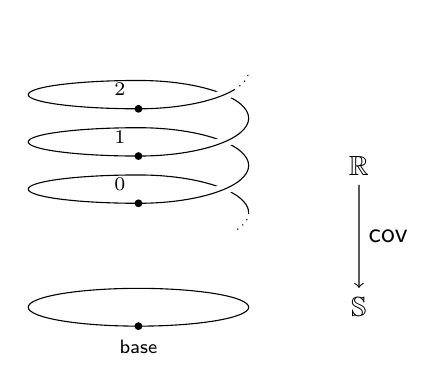
\begin{tikzpicture}[xscale=1.4,yscale=.6]
    \node (R) at (2,1) {$\mathbb{R}$};
    \node (S1) at (2,-2) {$\Sn$};
    \draw[->] (R) -- node[auto] {$\cov$} (S1);
    \draw (0,-2) ellipse (1 and .4);
    \draw[dotted] (1,0) arc (0:-30:1 and .8);
    \draw (1,0) arc (0:90:1 and .8) arc (90:270:1 and .3) coordinate (t1);
    \draw[white,line width=4pt] (t1) arc (-90:90:1 and .8);
    \draw (t1) arc (-90:90:1 and .8) arc (90:270:1 and .3) coordinate (t2);
    \draw[white,line width=4pt] (t2) arc (-90:90:1 and .8);
    \draw (t2) arc (-90:90:1 and .8) arc (90:270:1 and .3) coordinate (t3);
    \draw[white,line width=4pt] (t3) arc (-90:90:1 and .8);
    \draw (t3) arc (-90:-30:1 and .8) coordinate (t4);
    \draw[dotted] (t4) arc (-30:0:1 and .8);
    \node[fill,circle,inner sep=1pt,label={below:\scriptsize $\base$}] at (0,-2.4) {};
    \node[fill,circle,inner sep=1pt,label={above left:\scriptsize 0}] at (0,.2) {};
    \node[fill,circle,inner sep=1pt,label={above left:\scriptsize 1}] at (0,1.2) {};
    \node[fill,circle,inner sep=1pt,label={above left:\scriptsize 2}] at (0,2.2) {};
  \end{tikzpicture}
  %\caption{The winding map in classical topology}\label{fig:winding}
\end{figure}
%\pause
%
%\begin{definition}[Universal Cover of $\Sn^1$]
This will be a dependent type over $\Sn$, i.e.\ a type family $$\cov : \Sn \to \U.$$
%, with 
%\begin{align*}
%    \cov(\base) &:= \Z \\
%    \cov(\lloop) &:= \ua(\suc).
%\end{align*}
%\end{definition}
%\end{frame}
%
%%%%%%%%%%%%%%%%%%%%%%%%%%%%%%%%%%%%%%%%%%%%%%%%%%%%%%%%%%%%%%%%%%
%\begin{frame}{The Univalence Axiom: How it works}

To define a type family
\[
\cov : \Sn \longrightarrow \U,
\]
by the recursion property of the circle, we just need the following data:
\begin{itemize}
\item a point $A:\U$
\item a loop $p : A\rightsquigarrow A$
\end{itemize}

%\pause
For the point $A$ we take the integers $\Z$.
%\pause

By Univalence, to give a loop $p : \Z\rightsquigarrow \Z$ in $\U$, it suffices to give an equivalence $\Z\simeq \Z$.%\pause

Since $\Z$ is a set, equivalences are just isomorphisms, so we can take the successor function
$\suc : \Z\cong\Z$.

%\end{frame}
%%%%%%%%%%%%%%%%%%%%%%%%%%%%%%%%%%%%%%%%%%%%%%%%%%%%%%%%%%%%%%%%%%
%\begin{frame}{The Univalence Axiom: How it works}
%
%%
%\begin{figure}\centering
%  \begin{tikzpicture}[xscale=1.4,yscale=.6]
%    \node (R) at (2,1) {$\mathbb{R}$};
%    \node (S1) at (2,-2) {$\Sn$};
%    \draw[->] (R) -- node[auto] {$\cov$} (S1);
%    \draw (0,-2) ellipse (1 and .4);
%    \draw[dotted] (1,0) arc (0:-30:1 and .8);
%    \draw (1,0) arc (0:90:1 and .8) arc (90:270:1 and .3) coordinate (t1);
%    \draw[white,line width=4pt] (t1) arc (-90:90:1 and .8);
%    \draw (t1) arc (-90:90:1 and .8) arc (90:270:1 and .3) coordinate (t2);
%    \draw[white,line width=4pt] (t2) arc (-90:90:1 and .8);
%    \draw (t2) arc (-90:90:1 and .8) arc (90:270:1 and .3) coordinate (t3);
%    \draw[white,line width=4pt] (t3) arc (-90:90:1 and .8);
%    \draw (t3) arc (-90:-30:1 and .8) coordinate (t4);
%    \draw[dotted] (t4) arc (-30:0:1 and .8);
%    \node[fill,circle,inner sep=1pt,label={below:\scriptsize $\base$}] at (0,-2.4) {};
%    \node[fill,circle,inner sep=1pt,label={above left:\scriptsize 0}] at (0,.2) {};
%    \node[fill,circle,inner sep=1pt,label={above left:\scriptsize 1}] at (0,1.2) {};
%    \node[fill,circle,inner sep=1pt,label={above left:\scriptsize 2}] at (0,2.2) {};
%  \end{tikzpicture}
%  %\caption{The winding map in classical topology}\label{fig:winding}
%\end{figure}
%

\begin{definition}[Universal Cover of $\Sn^1$]
The dependent type $\cov : \Sn \to \U$ is given by circle-recursion, with 
\begin{align*}
    \cov(\base) &:= \Z \\
    \cov(\lloop) &:= \ua(\suc).
\end{align*}
\end{definition}

%\end{frame}
%%%%%%%%%%%%%%%%%%%%%%%%%%%%%%%%%%%%%%%%%%%%%%%%%%%%%%%%%%%%%%%%%
%%%%%%%%%%%%%%%%%%%%%%%%%%%%%%%%%%%%%%%%%%%%%%%%%%%%%%%%%%%%%%%%%%
%\begin{frame}{The Univalence Axiom: How it works}

%%
%\begin{figure}\centering
%  \begin{tikzpicture}[xscale=1.4,yscale=.6]
%    \node (R) at (2,1) {$\mathbb{R}$};
%    \node (S1) at (2,-2) {$\Sn$};
%    \draw[->] (R) -- node[auto] {$\cov$} (S1);
%    \draw (0,-2) ellipse (1 and .4);
%    \draw[dotted] (1,0) arc (0:-30:1 and .8);
%    \draw (1,0) arc (0:90:1 and .8) arc (90:270:1 and .3) coordinate (t1);
%    \draw[white,line width=4pt] (t1) arc (-90:90:1 and .8);
%    \draw (t1) arc (-90:90:1 and .8) arc (90:270:1 and .3) coordinate (t2);
%    \draw[white,line width=4pt] (t2) arc (-90:90:1 and .8);
%    \draw (t2) arc (-90:90:1 and .8) arc (90:270:1 and .3) coordinate (t3);
%    \draw[white,line width=4pt] (t3) arc (-90:90:1 and .8);
%    \draw (t3) arc (-90:-30:1 and .8) coordinate (t4);
%    \draw[dotted] (t4) arc (-30:0:1 and .8);
%    \node[fill,circle,inner sep=1pt,label={below:\scriptsize $\base$}] at (0,-2.4) {};
%    \node[fill,circle,inner sep=1pt,label={above left:\scriptsize 0}] at (0,.2) {};
%    \node[fill,circle,inner sep=1pt,label={above left:\scriptsize 1}] at (0,1.2) {};
%    \node[fill,circle,inner sep=1pt,label={above left:\scriptsize 2}] at (0,2.2) {};
%  \end{tikzpicture}
%  %\caption{The winding map in classical topology}\label{fig:winding}
%\end{figure}
%

As in classical homotopy theory, we use the universal cover to define the ``winding number" of any path $p : \base\rightsquigarrow\base$ by $\mathsf{wind}(p)=p_*(0)$. %\pause
 This gives a map
\[
\mathsf{wind} : \Omega(\Sn)\to\Z,
\]
which is inverse to the map $\Z\to\Omega(\Sn)$ given by
\[
z \mapsto \lloop^z.
\]

%\end{frame}
%%%%%%%%%%%%%%%%%%%%%%%%%%%%%%%%%%%%%%%%%%%%%%%%%%%%%%%%%%%%%%%%
%%%%%%%%%%%%%%%%%%%%%%%%%%%%%%%%%%%%%%%%%%%%%%%%%%%%%%%%%%%%%%%%
%
%\subsection*{The formal proof}
%%{\relsize{-15}
%\begin{verbatim}
%(* Theorems about the circle S^1. *)
%
%Require Import Overture PathGroupoids Equivalences Trunc HSet.
%Require Import Paths Forall Arrow Universe Empty Unit.
%Local Open Scope path_scope.
%Local Open Scope equiv_scope.
%Generalizable Variables X A B f g n.
%
%(* Definition of the circle. *)
%
%Module Export Circle.
%
%Local Inductive S1 : Type := 
%| base : S1.
%
%Axiom loop : base = base.
%
%Definition S1_rect (P : S1 -> Type) (b : P base) (l : loop # b = b)
%  : forall (x:S1), P x
%  := fun x => match x with base => b end.
%
%Axiom S1_rect_beta_loop
%  : forall (P : S1 -> Type) (b : P base) (l : loop # b = b),
%  apD (S1_rect P b l) loop = l.
%
%End Circle.
%
%(* The non-dependent eliminator *)
%
%Definition S1_rectnd (P : Type) (b : P) (l : b = b)
%  : S1 -> P
%  := S1_rect (fun _ => P) b (transport_const _ _ @ l).
%
%Definition S1_rectnd_beta_loop (P : Type) (b : P) (l : b = b)
%  : ap (S1_rectnd P b l) loop = l.
%Proof.
%  unfold S1_rectnd.
%  refine (cancelL (transport_const loop b) _ _ _).
%  refine ((apD_const (S1_rect (fun _ => P) b _) loop)^ @ _).
%  refine (S1_rect_beta_loop (fun _ => P) _ _).
%Defined.
%
%(* The loop space of the circle is the Integers. *)
%(* First we define the appropriate integers. *)
%
%Inductive Pos : Type :=
%| one : Pos
%| succ_pos : Pos -> Pos.
%
%Definition one_neq_succ_pos (z : Pos) : ~ (one = succ_pos z)
%  := fun p => transport (fun s => match s with one => Unit | succ_pos t 
%  => Empty end) p tt.
%
%Definition succ_pos_injective {z w : Pos} (p : succ_pos z = succ_pos w) : z = w
%  := transport (fun s => z = (match s with one => w | succ_pos a 
%  => a end)) p (idpath z).
%
%Inductive Int : Type :=
%| neg : Pos -> Int
%| zero : Int
%| pos : Pos -> Int.
%
%Definition neg_injective {z w : Pos} (p : neg z = neg w) : z = w
%  := transport (fun s => z = (match s with neg a => a | zero => w | pos a 
%  => w end)) p (idpath z).
%
%Definition pos_injective {z w : Pos} (p : pos z = pos w) : z = w
%  := transport (fun s => z = (match s with neg a => w | zero => w | pos a 
%  => a end)) p (idpath z).
%
%Definition neg_neq_zero {z : Pos} : ~ (neg z = zero)
%  := fun p => transport (fun s => match s with neg a => z = a | zero => Empty 
%  | pos _ => Empty end) p (idpath z).
%
%Definition pos_neq_zero {z : Pos} : ~ (pos z = zero)
%  := fun p => transport (fun s => match s with pos a => z = a 
%  | zero => Empty | neg _ => Empty end) p (idpath z).
%
%Definition neg_neq_pos {z w : Pos} : ~ (neg z = pos w)
%  := fun p => transport (fun s => match s with neg a => z = a 
%  | zero => Empty | pos _ => Empty end) p (idpath z).
%
%(* And prove that they are a set. *)
%
%Instance hset_int : IsHSet Int.
%Proof.
%  apply hset_decidable.
%  intros [n | | n] [m | | m].
%  revert m; induction n as [|n IHn]; intros m; induction m as [|m IHm].
%  exact (inl 1).
%  exact (inr (fun p => one_neq_succ_pos _ (neg_injective p))).
%  exact (inr (fun p => one_neq_succ_pos _ (symmetry _ _ (neg_injective p)))).
%  destruct (IHn m) as [p | np].
%  exact (inl (ap neg (ap succ_pos (neg_injective p)))).
%  exact (inr (fun p => np (ap neg (succ_pos_injective (neg_injective p))))).
%  exact (inr neg_neq_zero).
%  exact (inr neg_neq_pos).
%  exact (inr (neg_neq_zero o symmetry _ _)).
%  exact (inl 1).
%  exact (inr (pos_neq_zero o symmetry _ _)).
%  exact (inr (neg_neq_pos o symmetry _ _)).
%  exact (inr pos_neq_zero).
%  revert m; induction n as [|n IHn]; intros m; induction m as [|m IHm].
%  exact (inl 1).
%  exact (inr (fun p => one_neq_succ_pos _ (pos_injective p))).
%  exact (inr (fun p => one_neq_succ_pos _ (symmetry _ _ (pos_injective p)))).
%  destruct (IHn m) as [p | np].
%  exact (inl (ap pos (ap succ_pos (pos_injective p)))).
%  exact (inr (fun p => np (ap pos (succ_pos_injective (pos_injective p))))).
%Defined.
%
%(* Successor is an autoequivalence of [Int]. *)
%
%Definition succ_int (z : Int) : Int
%  := match z with
%       | neg (succ_pos n) => neg n
%       | neg one => zero
%       | zero => pos one
%       | pos n => pos (succ_pos n)
%     end.
%
%Definition pred_int (z : Int) : Int
%  := match z with
%       | neg n => neg (succ_pos n)
%       | zero => neg one
%       | pos one => zero
%       | pos (succ_pos n) => pos n
%     end.
%
%Instance isequiv_succ_int : IsEquiv succ_int
%  := isequiv_adjointify succ_int pred_int _ _.
%Proof.
%  intros [[|n] | | [|n]]; reflexivity.
%  intros [[|n] | | [|n]]; reflexivity.
%Defined.
%
%(* Now we do the encode/decode. *)
%
%Section AssumeUnivalence.
%Context `{Univalence} `{Funext}.
%
%Definition S1_code : S1 -> Type
%  := S1_rectnd Type Int (path_universe succ_int).
%
%(* Transporting in the codes fibration is the successor autoequivalence. *)
%
%Definition transport_S1_code_loop (z : Int)
%  : transport S1_code loop z = succ_int z.
%Proof.
%  refine (transport_compose idmap S1_code loop z @ _).
%  unfold S1_code; rewrite S1_rectnd_beta_loop.
%  apply transport_path_universe.
%Defined.
%
%Definition transport_S1_code_loopV (z : Int)
%  : transport S1_code loop^ z = pred_int z.
%Proof.
%  refine (transport_compose idmap S1_code loop^ z @ _).
%  rewrite ap_V.
%  unfold S1_code; rewrite S1_rectnd_beta_loop.
%  rewrite <- path_universe_V.
%  apply transport_path_universe.
%Defined.
%
%(* Encode by transporting *)
%
%Definition S1_encode (x:S1) : (base = x) -> S1_code x
%  := fun p => p # zero.
%
%(* Decode by iterating loop. *)
%
%Fixpoint loopexp {A : Type} {x : A} (p : x = x) (n : Pos) : (x = x)
%  := match n with
%       | one => p
%       | succ_pos n => loopexp p n @ p
%     end.
%
%Definition looptothe (z : Int) : (base = base)
%  := match z with
%       | neg n => loopexp (loop^) n
%       | zero => 1
%       | pos n => loopexp (loop) n
%     end.
%
%Definition S1_decode (x:S1) : S1_code x -> (base = x).
%Proof.
%  revert x; refine (S1_rect (fun x => S1_code x -> base = x) looptothe _).
%  apply path_forall; intros z; simpl in z.
%  refine (transport_arrow _ _ _ @ _).
%  refine (transport_paths_r loop _ @ _).
%  rewrite transport_S1_code_loopV.
%  destruct z as [[|n] | | [|n]]; simpl.
%  by apply concat_pV_p.
%  by apply concat_pV_p.
%  by apply concat_Vp.
%  by apply concat_1p.
%  reflexivity.
%Defined.
%
%(* The nontrivial part of the proof that decode and encode are equivalences 
%is showing that decoding followed by encoding 
%is the identity on the fibers over [base]. *)
%
%Definition S1_encode_looptothe (z:Int)
%  : S1_encode base (looptothe z) = z.
%Proof.
%  destruct z as [n | | n]; unfold S1_encode.
%  induction n; simpl in *.
%  refine (moveR_transport_V _ loop _ _ _).
%  by apply symmetry, transport_S1_code_loop.
%  rewrite transport_pp.
%  refine (moveR_transport_V _ loop _ _ _).
%  refine (_ @ (transport_S1_code_loop _)^).
%  assumption.
%  reflexivity.
%  induction n; simpl in *.
%  by apply transport_S1_code_loop.
%  rewrite transport_pp.
%  refine (moveR_transport_p _ loop _ _ _).
%  refine (_ @ (transport_S1_code_loopV _)^).
%  assumption.
%Defined.
%
%(* Now we put it together. *)
%
%Definition S1_encode_isequiv (x:S1) : IsEquiv (S1_encode x).
%Proof.
%  refine (isequiv_adjointify (S1_encode x) (S1_decode x) _ _).
%  (* Here we induct on [x:S1].  We just did the case when [x] is [base]. *)
%  refine (S1_rect (fun x => Sect (S1_decode x) (S1_encode x))
%    S1_encode_looptothe _ _).
%  (* What remains is easy since [Int] is known to be a set. *)
%  by apply path_forall; intros z; apply set_path2.
%  (* The other side is trivial by path induction. *)
%  intros []; reflexivity.
%Defined.
%
%Definition equiv_loopS1_int : (base = base) <~> Int
%  := BuildEquiv _ _ (S1_encode base) (S1_encode_isequiv base).
%
%End AssumeUnivalence.
%\end{verbatim}
%
%%\end{frame}
%%%%%%%%%%%%%%%%%%%%%%%%%%%%%%%%%%%%%%%%%%%%%%%%%%%%%%%%%%%%%%%%%
\subsection*{Formalization of mathematics}

\begin{itemize}
\item The idea of logical foundations of math has great conceptual and philosophical interest, but in the past this was too lengthy and cumbersome to be of any use.
%\pause

\item Explicit formalization of math is finally \emph{feasible}, because computers can now take over what was once too tedious or complicated to be done by hand.
%\pause

\item Future historians of mathematics will wonder how Frege and Russell could have invented formal logical foundations \emph{before} there were any computers to run them on!
%%\pause

\item Formalization can provide a \emph{practical tool} for working mathematicians and scientists: increased certainty and precision, supports collaborative work, cumulativity of results, searchable library of code, ... I think that mathematics will  eventually be fully formalized.
%\pause

\item UF uses a ``synthetic" method involving high-level axiomatics and structural descriptions; allows shorter, more abstract proofs; closer to mathematical practice than the ``analytic" method of ZFC.  Use of UA is very powerful.

\end{itemize}

\subsection*{Final Example: The cumulative hierarchy}

Given a universe $\U$, we can make the \emph{cumulative hierarchy} $V$ of sets  in $\U$ as a HIT:
\begin{itemize}
\item for any small  $A$ and any map $f : A\arr V$, there is a ``set":
\[
\mathsf{set}(A,f) : V
\]
We think of $\mathsf{set}(A,f)$ as the image of $A$ under $f$, i.e.\ the classical set $\{ f(a)\ |\ a \in A \}$

\item For all $A, B : \U$, $f : A \arr V$ and $g : B \arr V$ such that
    %
    \[
      \big(\forall{a:A}\,\exists{b:B}\ f(a) = g(b)\big) \wedge \big(\forall{b:B}\,\exists{a:A}\ f(a)=g(b)\big)
    \]
    %
    we put in a path in $V$ from $\mathsf{set}(A,f)$ to $\mathsf{set}(B,g)$.
  \item The $0$-truncation constructor: for all $x,y:V$ and $p,q:x=y$, we have $p=q$.
\end{itemize}

%\end{frame}
%%%%%%%%%%%%%%%%%%%%%%%%%%%%%%%%%%%%%%%%%%%%%%%%%%%%%%%%%%%%%%%%%
%\begin{frame}{The cumulative hierarchy of sets}

Membership $x\in y$ is then defined for elements of $V$ by:
\[
  (x \in \mathsf{set}(A,f))\ :=\  (\exists{a : A}.\ x = f(a)).
\]
%\pause

One can show that the resulting structure $(V,\in)$ satisfies most of the axioms of Aczel's constructive set theory CZF.
%\pause
%\medskip

Assuming AC for sets ($0$-types), one gets a model of ZFC set theory.
%\pause
%\medskip

The proofs make essential use of UA.
%\end{frame}


%\end{frame}
%%%%%%%%%%%%%%%%%%%%%%%%%%%%%%%%%%%%%%%%%%%%%%%%%%%%%%%%%
%%%%%%%%%%%%%%%%%%%%%%%%%%%%%%%%%%%%%%%%%%%%%%%%%%%%%%%%%%%%%%%
%\begin{frame}{Conclusion}
%
%\emph{\myemph{Homotopy Type Theory} is a topological interpretation of constructive type theory that allows purely formal reasoning in homotopy theory.}
%%\pause
%
%\medskip
%
%\emph{\myemph{Univalent Foundations} is a new approach to the foundations of mathematics based on \emph{Homotopy Type Theory}, with both intrinsic geometric content and a computational implementation.  }
%%\pause
%
%\medskip
%
%\emph{\myemph{The Univalence Axiom} is a powerful new principle of reasoning that is incompatible with conventional foundations, and yet (conjecture!) computationally admissible.}
%
%
%\end{frame}
%
%%%%%%%%%%%%%%%%%%%%%%%%%%%%%%%%%%%%%%%%%%%%%%%%%%%%%%%%%%%%%%
\subsection*{References and Further Information}

More Information:
\begin{center}
\tt{www.HomotopyTypeTheory.org}\\
\end{center}
\bigskip

%Current state of the Univalent Foundations Program:
%\begin{center}
%\tt{uf-ias-2012.wikispaces.com}
%\end{center}

The Book:
\begin{center}
\emph{Homotopy Type Theory: Univalent Foundations of Mathematics}\\
The Univalent Foundations Program,\\
 Institute for Advanced Study, 
 Princeton, 2013
\end{center}

%\end{frame}
%%%%%%%%%%%%%%%%%%%%%%%%%%%%%%%%%%%%%%%%%%%%%%%%%%%%%%%%%%%%%%%
%{
%\setbeamercolor{background canvas}{bg=}
%\includepdf{hottcover.pdf}
%}
%%%%%%%%%%%%%%%%%%%%%%%%%%%%%%%%%%%%%%%%%%%%%%%%%%%%%%%%%%%%%%%%%%%%%%

%%
\end{document}
%%
